\section{Anforderungsspezifikation}
\subsection{Allgemeine Beschreibung}
Generell sind zwei Anwendungsszenarien denkbar:
\begin{itemize}
	\item VPN-Client
	\item VPN-Server
\end{itemize}
\medskip
Dabei ist der VPN-Client eine \textbf{Muss}-Anforderung und der VPN-Server eine \textbf{Kann}-Anforderung.
\medskip
\subsubsection{VPN-Client}
Die Applikation wird von einem Standard-Nutzer verwendet. Dieser soll VPN Tunnels zu einem Servern konfigurieren können, diesen starten und stoppen. Die Konfigurationsmöglichkeiten sind beschränkt, als Vorlage wird der strongSwan Android Client verwendet.\\


\subsubsection{VPN-Server}
Der Server ist auf Systemadministratoren ausgerichtet. Es soll möglich sein, die VPN-Tunnels von strongSwan per grafischem Interface auf einem Server/Gateway zu konfigurieren.

\subsection{Use Case}
\subsubsection{Aktoren und Stakeholder}
\begin{table}[H]
\centering
    \begin{tabular}{|p{3cm}|p{9cm}|}
    \hline
    \rowcolor{lightblue}
    Aktor & Tätigkeit   \\ \hline
	User  & 
			\begin{itemize}
			\item Konfiguriert VPN-Tunnel als Client
    		\item Startet und stoppt VPN-Tunnel
		\end{itemize}	
	\\ \hline
	Administrator & 
			\begin{itemize}
			\item Konfiguriert VPN-Tunnel als Server
    		\item Startet und stoppt VPN-Tunnel
		\end{itemize}	
	\\ \hline
	\end{tabular}
    \caption[Aktoren und Stakeholder]{Aktoren und Stakeholder}
\end{table}




\subsubsection{Use Case Diagramm}
\begin{figure}[H]
\centering
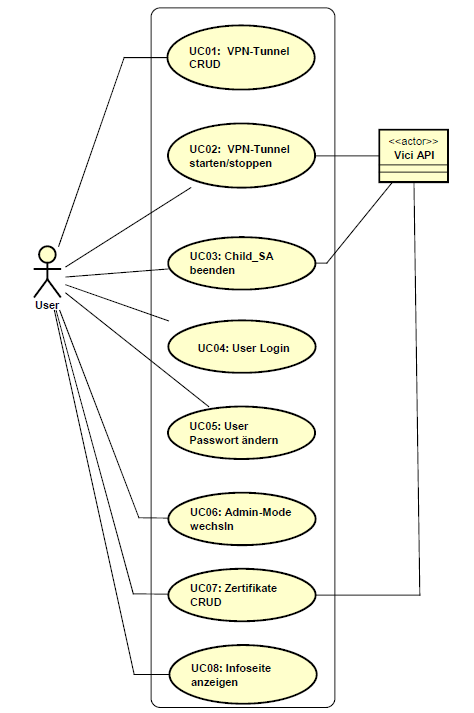
\includegraphics[width=350pt]{images/strongMan_usecase.png}
\caption[Use Case Diagramm]{Use Case Diagramm}
\end{figure}


\subsubsection{Use Cases Brief}
Alle hier definierten Use Cases haben auch ein entsprechendes Mockup im Anhang.
\paragraph{UC01: VPN-Tunnel CRUD}\mbox{} \\
Der User kann einen VPN-Tunnel erfassen / konfigurieren. Dabei hat er eine Auswahl von verschiedenen vordefinierten Authentisierungsmethoden. Jede Authentisierungsmethode hat vordefinierte Konfigurationsfelder, die der User ausfüllen muss. Die Tunnel-Übersichtsseite stellt die Hauptseite der Applikation dar. Dort können die Tunnels bearbeitet und gelöscht werden.

\paragraph{UC02: VPN-Tunnel starten/stoppen}\mbox{} \\
Der User kann einen erfassten VPN-Tunnel starten und stoppen. Dabei wird die Konfiguration über die Vici-Schnittstelle geladen. Falls ein VPN-Tunnel nicht aufgebaut werden kann, soll eine passende Fehlermeldung angezeigt werden. 

\paragraph{UC03: Child\_SA beenden}\mbox{} \\
Jeder VPN-Tunnel kann mehrere Child\_SA aufbauen. Diese werden in der Hauptseite angezeigt und können vom User beendet werden. Auch dieser Use Case interagiert mit der Vici-Schnittstelle. Nur im Server Modus.

\paragraph{UC04: User Login}\mbox{} \\
Der User loggt sich zu Beginn des Webseiten Aufrufs mit einem Usernamen und Passwort ein. Es existiert nur ein Benutzer.

\paragraph{UC05: User Passwort ändern}\mbox{} \\
Sobald der User eingeloggt ist, hat er die Möglichkeit, sein Passwort zu ändern. Dabei gibt er sein altes Passwort einmal und sein neues Passwort zweimal an.

\paragraph{UC06: Admin-Mode wechseln}\mbox{} \\
\textbf{Optional:} Das Userinterface unterscheidet zwischen zwei Modis: User- \& Admin-Mode. Der Modus soll über das Userinterface wechselbar sein. Der Admin-Mode stellt einige Server-spezifische Funktionalitäten zusätzlich zur Verfügung, welche der User zur einfacheren Bedienung nicht sieht. Nur im Server Modus.

\paragraph{UC07: Zertifikate CRUD}\mbox{} \\
Dem User wird eine Zertifikatsverwaltung zur Verfügung gestellt. Er kann Zertifikate und private Schlüssel in den gängigen Formaten uploaden, anschauen, updaten (Passwort ändern) und wieder löschen. Die Dateien können mit einem Passwort verschlüsselt sein. 

\paragraph{UC08: Infoseite anzeigen}\mbox{} \\
Die Informationsseite zeigt dem eingeloggten User verschieden Informationen des strongSwans zum Beispiel Version, installierte Plugins usw.

\newpage




